%% ============================================================
%% CHAPTER 4 — CVaR-Based Fair Deepfake Detection: DAG-FDD and DAW-FDD
%% ============================================================

\chapter{CVaR-Based Fair Deepfake Detection: DAG-FDD and DAW-FDD}
\label{ch:cvar_deepfake}



\vspace{0.5em}
\noindent\rule{\textwidth}{0.4pt}
\textbf{Declaration of Contributions:} This chapter was primarily authored by \textit{Aryan Choudhary}, who conducted a detailed study of the referenced work, systematically extracted its mathematical formulations and reformulated the methodology into this report chapter. The presentation of CVaR-based robust optimization along with demographic-agnostic and demographic-aware fairness frameworks was carefully structured and formalized to align with the objectives of the literature review. All mathematical expressions and derivations were rigorously verified to ensure consistency with the original paper.
\noindent\rule{\textwidth}{0.4pt}
\vspace{1em}

\bigskip
% ------------------------------------------------------------------ 
\section{Introduction}
\label{sec:ch4_intro}
% ------------------------------------------------------------------

In this chapter, we review the fairness oriented deepfake detection framework proposed in \cite{dag_paper}, with particular emphasis on the role of Conditional Value-at-Risk (CVaR) in robust optimisation. The central idea is that conventional training, which minimises average loss, tends to prioritise easy and dominant samples. In deepfake detection, this can lead to uneven performance across hidden or explicit demographic groups: a model may achieve strong overall accuracy while still producing substantially higher error rates for certain subpopulations.

To address this limitation, the paper introduces two related training strategies:

\begin{itemize}
    \item \textbf{DAG-FDD} (Demographic-Agnostic Fair Deepfake Detection) : used when demographic labels are \emph{not} available.
    \item \textbf{DAW-FDD} (Demographic-Aware Fair Deepfake Detection) : used when demographic labels \emph{are} available.
\end{itemize}

Both methods are built on the same broad principle: instead of optimising the average loss over all samples, the training procedure is modified to emphasise the worst-performing samples or groups. This makes the detector more robust and in the fairness setting, reduces the likelihood that the model performs well only on majority or easy cases. 

The contribution of this paper \cite{dag_paper} is particularly significant as it demonstrates that fairness can be incorporated through the objective function without requiring changes to the underlying detection architecture. Since the fairness behavior is largely governed by the loss formulation, the approach remains flexible and can be extended to a wide range of models.


% ------------------------------------------------------------------
\section{Background: Why Average Loss Is Not Enough}
\label{sec:ch4_avg_loss}
% ------------------------------------------------------------------

Standard learning methods minimise the expected loss

\begin{equation}
    R_{\mathrm{avg}}(\theta)
    = \mathbb{E}_{(X,Y)\sim P}\bigl[\ell(\theta;\,X,Y)\bigr],
    \label{eq:avg_risk}
\end{equation}

\noindent where $\theta$ denotes the model parameters, $(X,Y)$ is a training sample drawn from data distribution $P$, and $\ell(\theta;X,Y)$ is the prediction loss. This objective treats every sample equally on average. While effective for ordinary accuracy maximisation, it is not suitable when the dataset contains imbalance across subgroups: a model can reduce its total average loss by doing well on dominant or easier samples, even if it performs poorly on minority or difficult groups.

This is exactly the limitation which we try to overcome. The authors of \cite{dag_paper} argue that fairness in deepfake detection should not be measured only through average behaviour, because the average can hide worst-case performance. A detector that fails badly on one group but performs well on others may still appear strong under standard metrics. Therefore, the paper replaces average-risk training with a \emph{robust risk} objective.

% ------------------------------------------------------------------
\section{CVaR as the Core Robustness Principle}
\label{sec:cvar_core}
% ------------------------------------------------------------------

The paper \cite{dag_paper} uses \textbf{Conditional Value-at-Risk (CVaR)} as the main robust optimisation tool. CVaR is a classical idea from risk-sensitive optimisation; it focuses on the \emph{tail} of the loss distribution rather than its mean. For a given parameter vector $\theta$, the CVaR objective is

\begin{equation}
    \mathrm{CVaR}_{\alpha}(\theta)
    = \inf_{\lambda \in \mathbb{R}}
      \left\{
        \lambda
        + \frac{1}{\alpha}\,
          \mathbb{E}_{(X,Y)\sim P}
          \bigl[\,[\ell(\theta;\,X,Y) - \lambda]_{+}\,\bigr]
      \right\}
    \label{eq:cvar}
\end{equation}

\textit{The notion of infimum has been formally introduced in Chapter~\ref{ch:background}.}


\noindent where $[a]_{+} = \max(0,\,a)$.

\subsection{Interpretation of the variables}
\label{subsec:cvar_vars}

Here, $\lambda$ is a threshold or pivot value. The expression $[\ell(\theta;X,Y)-\lambda]_{+}$ retains only the part of the loss that exceeds $\lambda$: samples whose losses are below the threshold contribute nothing, while samples above the threshold contribute proportionally to how badly the model performs on them.

The parameter $\alpha \in (0,1)$ determines the fraction of the highest-loss region that is emphasised. A smaller $\alpha$ concentrates more strongly on the hardest samples, while a larger $\alpha$ makes the objective closer to average loss. This makes $\alpha$ an important hyperparameter in controlling how \emph{aggressively} the model focuses on the difficult portion of the data.

\subsection{Intuition}
\label{subsec:cvar_intuition}

The intuition behind CVaR is simple but powerful: instead of asking ``How well does the model perform on average?'', it asks ``How bad is the model on the worst fraction of cases?'' This is especially useful in fairness-sensitive applications, because the worst fraction of cases is often where minority or underrepresented groups appear.

% ------------------------------------------------------------------
\section{DAG-FDD: Demographic-Agnostic Fair Deepfake Detection}
\label{sec:dag_fdd}
% ------------------------------------------------------------------

\subsection{Motivation}
\label{subsec:dag_motivation}

DAG-FDD is used when demographic labels are not available which is a realistic scenario in many deepfake detection settings, since training sets may not contain explicit annotations for race, sex, age or other sensitive attributes. Even without demographic labels, the data may still contain \emph{latent groups}, some of which may be harder to classify than others. DAG-FDD is designed to reduce the risk that the detector performs disproportionately poorly on such hidden subgroups.

\subsection{Latent-Group Formulation}
\label{subsec:dag_latent}

The paper models the overall data distribution as a mixture of $K$ latent group distributions:

\begin{equation}
    P = \sum_{m=1}^{K} \pi_m\, P_m
    \label{eq:mixture}
\end{equation}

\noindent where $P_m$ is the distribution of the $m$-th latent group, $\pi_m$ is its mixture weight, and $\sum_m \pi_m = 1$. The corresponding worst-group risk is

\begin{equation}
    R_{\max}(\theta)
    = \max_{m=1,\ldots,K}\;
      \mathbb{E}_{(X,Y)\sim P_m}\bigl[\ell(\theta;\,X,Y)\bigr]
    \label{eq:worst_group_risk}
\end{equation}

This objective directly represents the fairness concern: instead of minimising the mean risk across all groups, we control the risk of the worst group.

\subsection{Why CVaR Helps in the Demographic-Agnostic Setting}
\label{subsec:dag_cvar_bound}

The paper \cite{dag_paper} shows that CVaR on sample losses can act as an upper-bound surrogate for worst-group risk when $\alpha$ is small enough. Specifically, if

\begin{equation}
    \alpha \;\leq\; \min_{m}\;\pi_m
    \label{eq:alpha_bound}
\end{equation}

\noindent then the CVaR objective provides an upper bound on the maximum group risk. This result is important because it justifies using sample-level CVaR even when group labels are missing. The practical meaning is that the hardest samples in the overall dataset tend to come from the hardest latent groups; therefore, if training is forced to pay greater attention to the worst samples, the model indirectly becomes more robust to hidden demographic imbalance.

\subsection{Empirical Objective Used in DAG-FDD}
\label{subsec:dag_objective}

For a dataset of size $n$, the empirical DAG-FDD objective is

\begin{equation}
    \mathcal{L}_{\mathrm{DAG\text{-}FDD}}(\theta,\lambda)
    = \lambda
      + \frac{1}{\alpha n}
        \sum_{i=1}^{n}
        \bigl[\ell(\theta;\,X_i,Y_i) - \lambda\bigr]_{+}
    \label{eq:dag_obj}
\end{equation}

\noindent This is the sample-based approximation of the population CVaR objective~\eqref{eq:cvar}. The term $\lambda$ sets the threshold level; the summation considers only samples whose loss exceeds the threshold; and the factor $1/(\alpha n)$ rescales the tail contribution so that the hardest samples dominate the update. In effect, DAG-FDD behaves like a principled version of hard-example mining.

\subsection{Optimisation of DAG-FDD}
\label{subsec:dag_optim}

The paper optimises DAG-FDD by alternating between the threshold parameter $\lambda$ and the model parameters $\theta$. For fixed $\theta$, the objective is convex in $\lambda$, so $\lambda$ can be found efficiently by binary search. For fixed $\lambda$, the model parameters are updated by gradient descent:

\begin{equation}
    \theta^{l+1}
    = \theta^{l}
      - \frac{\eta}{\alpha\,|S_b|}
        \sum_{i \in S_b}
        \frac{\partial}{\partial\theta}\,\ell(\theta^l;\,X_i,Y_i)
        \cdot
        \mathbf{1}\bigl[\ell(\theta^l;\,X_i,Y_i) > \lambda\bigr]
    \label{eq:dag_grad}
\end{equation}

\noindent where $S_b$ is the mini-batch, $\eta$ is the learning rate, and $\mathbf{1}[\cdot]$ is the indicator function. Only the samples with losses above the threshold contribute to the gradient. 

\emph{It is the main mechanism by which DAG-FDD shifts learning towards difficult samples.}

\subsection{Interpretation}
\label{subsec:dag_interp}

The demographic-agnostic setting is especially useful because it does not require any sensitive labels, making the method broadly applicable. The fairness guarantee is indirect: the method cannot guarantee equality across explicit groups because those groups are not known. Instead, it controls the worst-case behaviour among latent subpopulations, still very valuable, since hidden demographic imbalance is common in real datasets.

% ------------------------------------------------------------------
\section{DAW-FDD: Demographic-Aware Fair Deepfake Detection}
\label{sec:daw_fdd}
% ------------------------------------------------------------------

\subsection{Motivation}
\label{subsec:daw_motivation}

DAW-FDD is used when demographic labels are available (e.g.\ race or sex labels). In this case, fairness can be enforced more explicitly and directly. Unlike DAG-FDD, which treats the data as a collection of unlabelled samples, DAW-FDD recognises the existence of demographic groups and explicitly tries to reduce performance disparity among them.

\subsection{Group Risk}
\label{subsec:daw_group_risk}

Let $\mathcal{G}$ denote the set of demographic groups. For a sample $i$ belonging to group $g$, the group-specific risk is

\begin{equation}
    R_g(\theta)
    = \mathbb{E}_{(X,Y)\mid G=g}\bigl[\ell(\theta;\,X,Y)\bigr]
    \label{eq:group_risk}
\end{equation}

\noindent The fairness goal is to avoid situations where some groups experience substantially larger risk than others, particularly important in deepfake detection, since a detector that is less accurate for one demographic group may amplify unfairness in downstream applications.

\subsection{Group-Level CVaR}
\label{subsec:daw_group_cvar}

The paper also introduces a CVaR objective over group risks \cite{dag_paper}:

\begin{equation}
    \mathrm{CVaR}_{\alpha}^{\mathcal{G}}(\theta)
    = \inf_{\lambda \in \mathbb{R}}
      \left\{
        \lambda
        + \frac{1}{\alpha}\,
          \mathbb{E}_{G \sim \mathrm{Uniform}(\mathcal{G})}
          \bigl[\,[R_g(\theta) - \lambda]_{+}\,\bigr]
      \right\}
    \label{eq:group_cvar}
\end{equation}

\noindent This differs from DAG-FDD in an important way: the quantity being evaluated is not the loss of individual samples, but the loss of entire groups. The method therefore places direct pressure on the worst-performing demographic groups. The paper further notes that the group-CVaR objective can be interpreted as balancing the average risk across groups and the deviation from the worst groups, so DAW-FDD actively suppresses disparity rather than merely optimising accuracy under group awareness.

% ------------------------------------------------------------------
\subsection{Per-Group Top \texorpdfstring{$k$}{k} / CVaR Estimation}
\label{sec:per_group_topk}
% ------------------------------------------------------------------

\subsubsection{Why an Additional Mechanism Is Needed}
\label{subsec:topk_motivation}

One major issue in the demographic-aware setting is that each group may itself contain an imbalanced class composition. For example, a group may have many more real samples than fake samples, or vice versa. If one simply averages losses within each group, the majority class may dominate the group-risk estimate. To address this, the paper introduces a top-$k$ (or CVaR-style) estimator \emph{inside} each group \cite{dag_paper}, ensuring that the hardest examples within a group contribute more strongly to the group loss.

\subsubsection{Group-Level Top \texorpdfstring{$k$}{k} Loss}
\label{subsec:topk_loss}

For a group $g$, the group loss is computed in a CVaR-equivalent form over the hardest fraction of its samples:

\begin{equation}
    \mathcal{L}_g(\theta)
    = \min_{\lambda_g \in \mathbb{R}}
      \left\{
        \lambda_g
        + \frac{1}{\alpha_g\, n_g}
          \sum_{i \in \mathcal{I}_g}
          \bigl[\ell(\theta;\,X_i,Y_i) - \lambda_g\bigr]_{+}
      \right\}
    \label{eq:group_topk}
\end{equation}

\noindent where $\mathcal{I}_g$ is the index set of samples in group $g$, $n_g = |\mathcal{I}_g|$, $\alpha_g$ controls how much of the group's tail is retained and $\lambda_g$ is a group-specific threshold.

\subsubsection{Role of \texorpdfstring{$\alpha_g$}{alpha\_g}}
\label{subsec:alpha_g_role}

The parameter $\alpha_g$ determines the degree of emphasis on the hardest samples within a group: a smaller value means only the worst examples are considered, while a larger value includes a broader portion of the group. In practice, $\alpha_g$ prevents a group's loss estimate from being diluted by easy or majority-class samples, especially important in deepfake detection, where the real/fake imbalance within each group can otherwise distort the fairness objective.

% ------------------------------------------------------------------
\subsection{Final DAW-FDD Objective}
\label{sec:daw_objective}
% ------------------------------------------------------------------

The overall DAW-FDD objective is \emph{hierarchical}. It first computes a robust loss within each group and then applies another CVaR layer over the groups themselves:

\begin{equation}
    \mathcal{L}_{\mathrm{DAW\text{-}FDD}}(\theta,\lambda)
    = \lambda
      + \frac{1}{\alpha\,|\mathcal{G}|}
        \sum_{g \in \mathcal{G}}
        \bigl[\mathcal{L}_g(\theta) - \lambda\bigr]_{+}
    \label{eq:daw_obj}
\end{equation}

\noindent where $\mathcal{L}_g(\theta)$ is given by Equation~\eqref{eq:group_topk}.

\subsubsection{How to Interpret the Two Levels}
\label{subsec:daw_two_levels}

This objective embeds two nested robustness mechanisms:

\begin{itemize}
    \item \textbf{Inner level:} within each demographic group, focus on the hardest samples.
    \item \textbf{Outer level:} across all groups, focus on the worst-performing groups.
\end{itemize}

\noindent DAW-FDD is therefore more structured than DAG-FDD. It does not merely emphasise hard samples globally, but explicitly separates the fairness problem into two levels: sample-level imbalance and group-level disparity.

\subsubsection{Optimisation Procedure}
\label{subsec:daw_optim}

The paper optimises DAW-FDD by alternating among three types of variables: the group thresholds $\lambda_g$, the global threshold $\lambda$, and the model parameters $\theta$. \emph{A sample contributes to the update only if it is hard relative to its group, and a group contributes strongly only if it is hard relative to the overall population.} This double filtering effect encourages fairness both \emph{within} and \emph{across} groups.

% ------------------------------------------------------------------
\section{Relationship Between DAG-FDD and DAW-FDD}
\label{sec:dag_vs_daw}
% ------------------------------------------------------------------

The two methods are closely related, but solve slightly different versions of the same fairness problem. Table~\ref{tab:dag_vs_daw} summarises the key differences.

\begin{table}[htbp]
\centering
\caption{Comparison of DAG-FDD and DAW-FDD.}
\label{tab:dag_vs_daw}
\begin{tabular}{@{}lll@{}}
\toprule
\textbf{Property} & \textbf{DAG-FDD} & \textbf{DAW-FDD} \\
\midrule
Demographic labels required & No  & Yes \\
Group structure assumed     & Latent (implicit) & Explicit \\
CVaR applied to             & Individual samples & Groups + samples \\
Fairness guarantee          & Worst latent group & Worst explicit group \\
Complexity                  & Lower & Higher (hierarchical) \\
\bottomrule
\end{tabular}
\end{table}

\noindent In summary, DAG-FDD can be viewed as a \emph{latent-group} robust optimisation method, whereas DAW-FDD is a \emph{hierarchical group-robust} optimisation method. The former protects against hidden worst-case behaviour; the latter protects against known demographic disparities. From a fairness perspective, DAW-FDD is more informative when group annotations are available, but DAG-FDD is more practical when such annotations are missing.

% ------------------------------------------------------------------
% ------------------------------------------------------------------
\section{Experimental Results Reported in the Paper}
\label{sec:ch4_experiments}
% ------------------------------------------------------------------

The experimental setup in \cite{dag_paper} is designed to evaluate whether CVaR-based objectives can improve fairness without degrading detection performance. The evaluation spans multiple datasets, architectures, and fairness settings.

\paragraph{Experimental Setup Overview}
\begin{itemize}
    \item \textbf{Datasets:} FaceForensics++ (FF++), Celeb-DF, DeepFakeDetection (DFD), and DFDC.
    \item \textbf{Backbones:} Xception, ResNet-50, EfficientNet-B3, DSP-FWA, and RECCE.
    \item \textbf{Fairness Metrics:} GFPR, FFPR, FEO (measuring group-wise false-positive disparities across gender, race and intersection).
    \item \textbf{Detection Metrics:} AUC, FPR, TPR, ACC
\end{itemize}

\noindent
A key design choice in the paper is the emphasis on \textbf{false-positive fairness}, since misclassifying real content as fake can have significant real-world consequences.

% ------------------------------------------------------------------
\subsection{Key Observations}
\label{subsec:ch4_main_results}
% ------------------------------------------------------------------

The results across all experiments exhibit several consistent trends:

\begin{itemize}
    \item \textbf{Fairness improvement is consistent:}  
    Both DAG-FDD and DAW-FDD reduce disparity in GFPR, FFPR and FEO across all datasets.

    \item \textbf{No strong fairness--accuracy trade-off:}  
    In multiple cases, detection performance (AUC, ACC) is preserved or even improved.

    \item \textbf{DAG vs DAW behaviour:}
    \begin{itemize}
        \item DAG-FDD performs well without demographic labels by focusing on hard samples.
        \item DAW-FDD performs better when labels are available due to explicit group-level optimisation.
    \end{itemize}

    \item \textbf{Intersectional fairness improves:}  
    Gains are not limited to single attributes; intersection groups (race + gender) also show reduced disparity.
\end{itemize}

% ------------------------------------------------------------------
\subsection{Results on FF++ (In-Domain Analysis)}
\label{subsec:ch4_ffpp}
% ------------------------------------------------------------------

\begin{figure}[htbp]
    \centering
    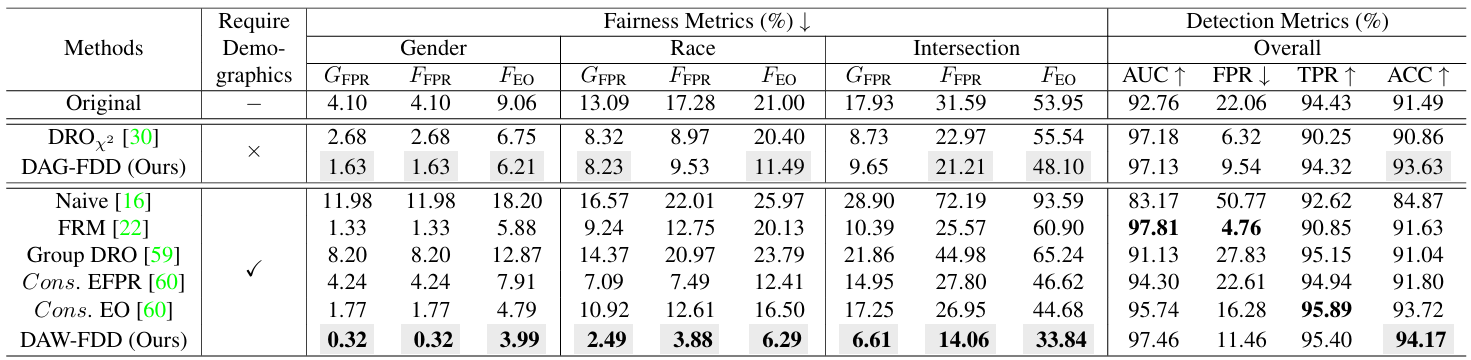
\includegraphics[width=\textwidth]{images/dag_img1.png}
    \caption{Comparison of fairness-aware methods on FF++ using the Xception backbone (adapted from \cite{dag_paper}).}
    \label{fig:ch4_ffpp_xception}
\end{figure}

\begin{figure}[htbp]
    \centering
    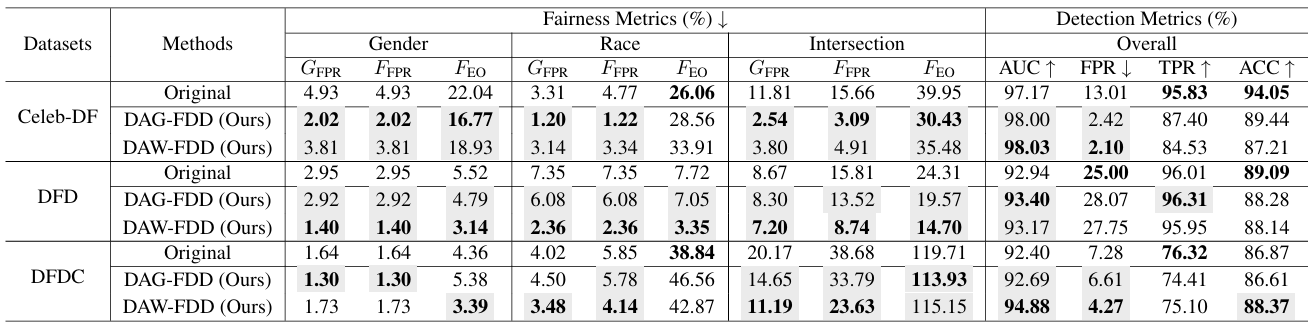
\includegraphics[width=\textwidth]{images/dag_img2.png}
    \caption{Evaluation on Celeb-DF, DFD, and DFDC using Xception (adapted from \cite{dag_paper}). Results show fairness and detection metrics across datasets.}
    \label{fig:ch4_dataset_comparison}
\end{figure}

From Figure~\ref{fig:ch4_ffpp_xception}, the following patterns can be observed:

\begin{itemize}
    \item \textbf{Strong reduction in fairness gaps:}  
    Both DAG-FDD and DAW-FDD significantly lower GFPR/FFPR compared to the original model.

    \item \textbf{DAW-FDD achieves best fairness:}  
    When demographic labels are available, DAW-FDD consistently produces the lowest group disparities.

    \item \textbf{Competitive detection performance:}  
    Improvements in fairness do not come at the cost of AUC or accuracy.

    \item \textbf{Comparison with prior fairness methods:}  
    The proposed methods outperform baselines such as DRO, Group DRO, and constraint-based approaches.
\end{itemize}

\noindent
This confirms that CVaR-based optimisation is effective even in standard in-domain training.

% ------------------------------------------------------------------
\subsection{Cross-Dataset Generalisation}
\label{subsec:ch4_crossdomain}
% ------------------------------------------------------------------

Figure~\ref{fig:ch4_dataset_comparison} evaluates generalisation across datasets.

\begin{itemize}
    \item \textbf{Fairness improvements persist across datasets:}  
    Both DAG-FDD and DAW-FDD continue to reduce disparity outside the training dataset.

    \item \textbf{Robustness to distribution shift:}  
    The method remains effective even when data characteristics change (e.g., DFDC vs FF++).

    \item \textbf{DAW-FDD benefits from group labels:}  
    When demographic structure is available, improvements are more pronounced.

    \item \textbf{DAG-FDD remains practical:}  
    Even without labels, DAG-FDD provides meaningful robustness gains.
\end{itemize}

\noindent
This indicates that the CVaR objective is not overfitting to a specific dataset distribution.

\begin{figure}[htbp]
    \centering
    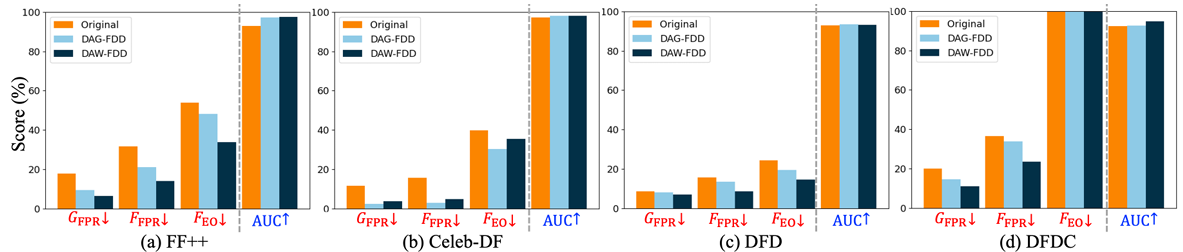
\includegraphics[width=\textwidth]{images/dag_img4.png}
    \caption{Intersectional fairness comparison of the Xception detector across four datasets: FF++, Celeb-DF, DFD, and DFDC (adapted from Figure~1 in \cite{dag_paper}).}
    \label{fig:ch4_intersection_multidataset}
\end{figure}

\begin{figure}[htbp]
    \centering
    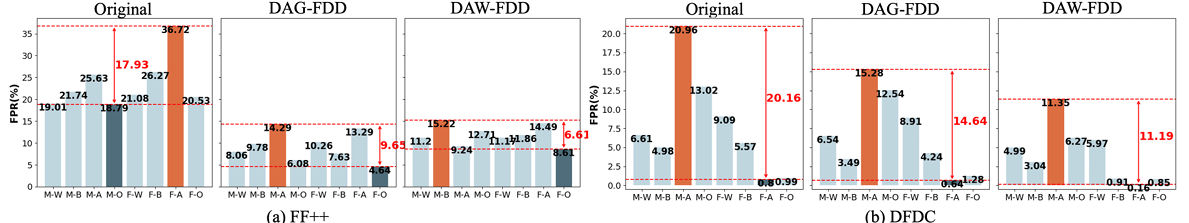
\includegraphics[width=\textwidth]{images/dag_img5.png}
    \caption{FPR comparison of the Xception detector on intersectional groups for FF++ and DFDC (adapted from Figure~2 in \cite{dag_paper}). Orange and dark cyan bars denote the groups with the highest and lowest FPR, respectively, and the red bracket shows the gap, where a smaller value is better.}
    \label{fig:ch4_intersection_fpr_gap}
\end{figure}

Figure~\ref{fig:ch4_intersection_multidataset} provides a more detailed view of the intersectional setting across datasets. It shows that the proposed methods consistently \emph{reduce the fairness gaps for intersection groups while maintaining competitive AUC}. The improvement is visible not only on FF++, but also on Celeb-DF, DFD, and DFDC, which supports the paper's claim that the CVaR-based objectives generalize well beyond a single benchmark.

Figure~\ref{fig:ch4_intersection_fpr_gap} focuses specifically on false-positive disparity across intersection groups. This is especially important because the paper emphasizes FPR as the most practically harmful error mode in deepfake detection. Both DAG-FDD and DAW-FDD reduce the gap between the highest and lowest FPR groups, showing that the fairness objective improves not just average behavior but also worst-group outcomes.

% ------------------------------------------------------------------
\subsection{Backbone Robustness}
\label{subsec:ch4_stability}
% ------------------------------------------------------------------

\begin{figure}[htbp]
    \centering
    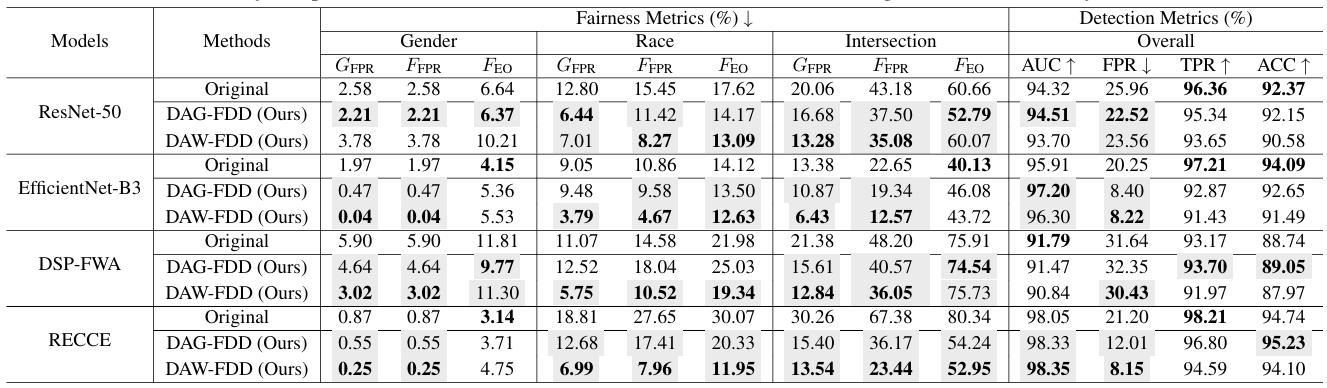
\includegraphics[width=\textwidth]{images/dag_img3.png}
    \caption{Performance across multiple backbones (ResNet-50, EfficientNet-B3, DSP-FWA, RECCE) on FF++ (adapted from \cite{dag_paper}).}
    \label{fig:ch4_backbone_comparison}
\end{figure}

Figure~\ref{fig:ch4_backbone_comparison} demonstrates that the proposed method is not tied to a specific architecture.

\begin{itemize}
    \item \textbf{Backbone-agnostic behaviour:}  
    Fairness improvements are consistent across all evaluated detectors.

    \item \textbf{Stable detection metrics:}  
    Performance remains competitive regardless of architecture.

    \item \textbf{Plug-and-play nature:}  
    The method only modifies the loss function and can be integrated into existing models.
\end{itemize}

% ------------------------------------------------------------------
\subsection{Computational Considerations}
\label{subsec:ch4_efficiency}
% ------------------------------------------------------------------

\begin{itemize}
    \item \textbf{Additional overhead:}  
    Comes from optimisation of CVaR thresholds ($\lambda$, $\lambda_g$).

    \item \textbf{Implementation cost:}  
    Requires binary search or iterative updates.

    \item \textbf{Practical trade-off:}  
    The overhead is modest relative to the fairness gains achieved.
\end{itemize}
 
% ------------------------------------------------------------------

\section{Key Insights for Our Project}
\label{sec:ch4_insights}
% ------------------------------------------------------------------

This paper is useful for our project because it offers a clean way to promote fairness without redesigning the full architecture. The main lesson we draw from it is that \textbf{fairness can be controlled at the optimisation level}. The most important takeaways are as follows.

\begin{enumerate}
    \item Worst-case focus is more informative than average loss when the goal is fair and robust performance.
    \item Hierarchical CVaR is a natural way to handle fairness when both sample-level hardness and group-level imbalance are present.
    \item DAG-FDD is the appropriate formulation when demographic labels are not available.
    \item DAW-FDD is the more structured and more explicit formulation when demographic labels are available.
    \item The top-$k$ or CVaR estimator inside each group is important for handling imbalance between real and fake samples within a demographic group.
\end{enumerate}

% ------------------------------------------------------------------
\section{Conclusion}
\label{sec:ch4_conclusion}
% ------------------------------------------------------------------

In this chapter, we described the CVaR-based fairness framework for deepfake detection and explained how it leads to two related methods: DAG-FDD and DAW-FDD. DAG-FDD handles the setting where demographic labels are absent and works through latent worst-case sample optimisation. DAW-FDD extends the same idea to the demographic-aware setting by adding group-level CVaR and per-group top-$k$ estimation.

The main contribution of the paper is that it replaces average-risk training with a more robust and fairness-sensitive objective, allowing the detector to pay greater attention to the hardest samples and the worst-performing groups, which in turn improves fairness without significantly compromising detection quality. For our own work, this paper serves as a strong reference for using robust optimisation as a fairness mechanism in deepfake detection.
